

\chapter{Swimmer Model}
\label{chap:chapter_2}

\section{Swimmers in Nature}
\label{sec:section_1}







\section{Swimmer Mechanics}
\label{sec:section 2}
The mechanics of swimmers is a complex problem\cite{tytell_interactions_2010}. The bodies of swimmers are elastic structures that deform in reaction to fluid forces but also affect the fluid around the swimmers.
In recent years, there were much progress in understanding the fluid motion around swimming bodies\cite{shadwick_fish_2006}, along with the nonlinear properties of muscle\cite{williams_new_2010} and the elastic behavior of 
swimmers bodies\cite{williams_new_2010}. Most of the studies performed with swimmers examined body mechanics separately from fluid mechanics, not including the coupled
fluid-structure interaction problem swimmers. Some Computational Fluid Dynamics (CFD) models have included some fluid-structure interaction, coupling center-of-mass motion to 
fluid dynamic forces with precribed body kinematics(\cite{kern_simulations_2006},\cite{borazjani_role_2010}).

\par

The swimmer configuration used in the simulations is described in Figure~\ref{fig:Bild1}. It is divided in three different parts: head, active tail and passive tail. The head 
is considered as an inactive region, that means no deformations are aplied in the bonds belonging to it. Also, the particles that belong to the head have a lower mass property
compared to the rest of the body to represent the head flesh softness. The active tail is the beating part of the tail, the propulsion of the swimmer is generated due to sinusoidal 
propagating wave in this part of the tail. The parameters defined to describe the beat pattern will be discussed later. The passive tail has the size of 2/9 of the total tail length
and it particles has the same mass properties as the active tail, but this fragment is passive and follows the active tail beat movements. 


\begin{figure}[ht]
  \centering
  \begin{footnotesize}
  \includegraphics[scale=0.25]{images/swimmer-struc.png}
  \caption[Swimmer Structure]{Swimmer structure}
  \label{fig:Bild1}
  \end{footnotesize}
\end{figure} 


In this model, the swimmer consists on particles which are connected by bonds and are arranged in a filamentous structure. These particle-bonds connections have a bead-spring 
structure (Figure~\ref{fig:Bild2}). Initially, all particles in the tail ( active and passive fragments) has the same mass $m$. The bond length $l_{b}$ between neighboring
particles and the distance between the parallel filaments are identical. The filament length and the distance between filaments is described by harmonic bond potentials between
the two beads (spring constant $K$).

\begin{figure}[ht]
  \centering
  \begin{footnotesize}
  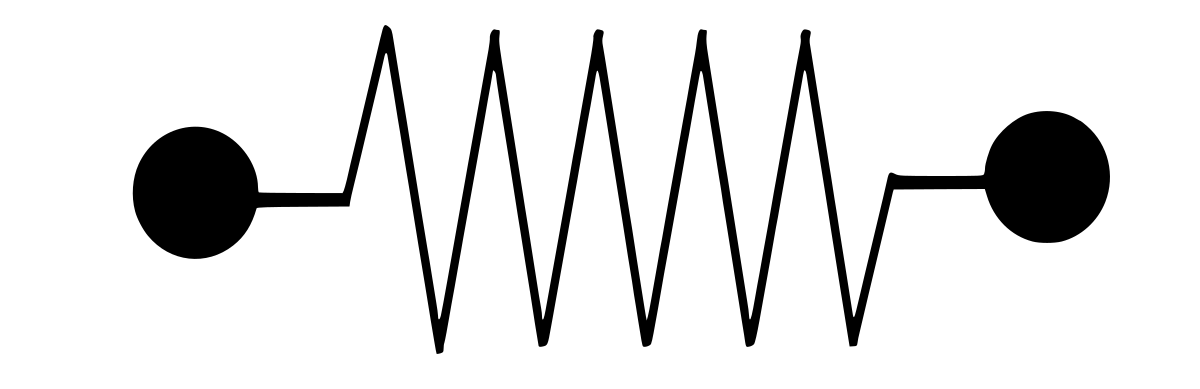
\includegraphics[scale=0.25]{images/bead-spring.png}
  \caption[Bead-Spring structure]{Bead-Spring structure}
  \label{fig:Bild2}
  \end{footnotesize}
\end{figure} 

For the simulations, the swimmer has a total number of 100 particles, where three of those forms the swimmer head. Initially, it was used a square form for the head due for 